\begin{figure}[t]
% \vspace{-5pt}
\centering
 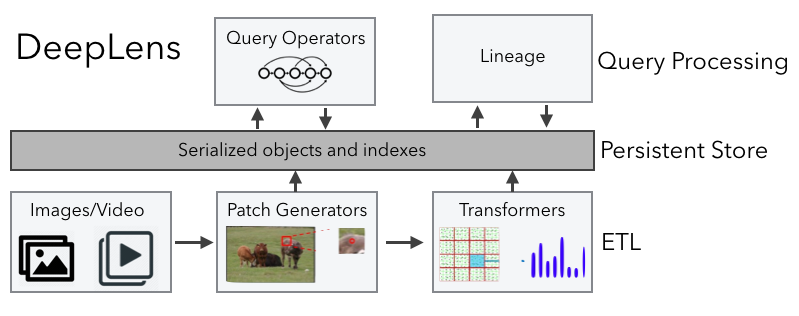
\includegraphics[width=\columnwidth]{figures/teaser.png}
 \caption{DeepLens has a dataflow-like architecture for processing visual analytics queries. All analysis is cast as relational queries on relations of image patches. Intermediate results can be materialized and indexed.  \label{teaser} }
\end{figure}

\section{DeepLens Architecture}
Our architecture is designed as a middle ground between the pure stateless dataflow approach and the RDBMS approach.
\textsf{DeepLens} provides dataflow operators to shape, transform, and manipulate image corpora at scale, but also supports materialization and indexing of intermediate results.
Figure \ref{teaser} illustrates the basic architecture with three main layers: (1) ETL, (2) Persistent Storage, and (3) Query Processing.

There are access methods which point to iterators over images derived from a filesystem or sampled from a video stream. The image dataflow is passed into a  \textbf{patch generator} that turns the image into a set of patches. Associated with each patch is a key-value dictionary storing metadata about how the patch was generated and any property of the patch. The patches are then fed into a composition of \textbf{transformers} that featurize, compress, or otherwise store detected properties of the patches into the dictionary. Over tuples of transformed patches, users can build a directed computation graph with \textbf{operators} (e.g., select, join).
Tuple-level lineage is automatically maintained by the system allowing any downstream patch to be associated with its base data.
Any of the intermediate results can be \textbf{materialized}. 
Furthermore, indexes can be built on any materialized data, either the key-value attributes or the image data.

\subsection{Visual ETL}
\label{subsection:visualETL}
In \textsf{DeepLens},  images reside in a filesystem or can be sampled from common video formats (e.g., MP4, OGG, etc.). Data are ingested into the system as 3-D dense arrays representing width and height of images, as well as  corresponding RGB channels. In a sense, this data is unstructured data. Semantics from image data have to be first extracted with computer vision algorithms before structured queries can be executed. 
The ETL layer defines the generation of \texttt{Patch} objects and their manipulation.

\vspace{0.25em}
\noindent \textbf{Patch Generators (Extract): } We provide a library of \texttt{Patch Generators}. 
These generators take as input an iterator over raw images and return an iterator over \texttt{Patch} objects.  
Our experiments consider three instantiations of these generators: object detection (ones that segment objects out of the image return segmentation masks), optical character recognition (one that identifies text in an image and returns a segmentation as well as the recognized string) and whole-image patches (returns the whole image).


\vspace{0.25em}
\noindent \textbf{Transformers (Transform): } The main content of patch is still raw pixel data, which is often not very useful on its own.
To be able to compare or manipulate the patches, we need a featurized representation.
This leads to the next module of the ETL layer which defines Transformers. 
A transformer take as input an iterator over \texttt{Patch} objects and returns an iterator over transformed \texttt{Patch} objects.  
In our experiments, we consider two transformers: color histogram features for image matching and a depth prediction neural network which predicts the 3D geometry of a patch. 

\vspace{0.25em}
\noindent \textbf{Materialize (Load): } \textsf{DeepLens} allows any stage of this pipeline to be materialized and persisted to disk or memory.

\subsection{Persistent Storage}
The persistent storage is implemented with BerkeleyDB\footnote{Implemented with bsddb3 (Python binding for BerkeleyDB)}. The image and feature data is serialized in a binary format before insertion. By default, the \texttt{Patches} are stored in a sorted file by record number (or frame number for videos). This is because many queries of interest examine particular time segments of videos.
The sorted file allows for quick retrieval of temporal predicates.

We also support the construction of indexes on the materialized data.
The challenge is that every data type requires a specialized index structure.
Over string valued or discrete metadata, the index choices are straight-forward. 
We support both hash tables and B+ trees are supported over any key (both of which are implemented with BerkeleyDB).

For the multidimensional data (patch segmentation parameters or image features), indexing is a little more nuanced and dependent on the workload.
As a concrete example, let us consider patches that are parametrized by ``bounding boxes'' (x1,y1,x2,y2).
Even though this data is multidimensional, we might effectively be interested in single dimensional queries.
For example, find bounding boxes left of a certain point in the image.
To support such queries, we found that it was far more efficient to use a B+ tree rather than an R-Tree multidimensional index.
On the other hand, if we are interested in containment and interesection queries, then we need a true multidimensional index.
We provide an interface to a disk-based R-Tree implemented with \texttt{libspatialindex}\footnote{https://libspatialindex.github.io/}.

However, we found that existing R-Tree implementations are optimized for geospatial problems in 2D.
They could not be efficiently modified for higher dimensional data.
This is exactly what we need for image matching queries, ones that compare features of two images and threshold the similarity.
For this class of queries and data, a data structure called a Ball-Tree was the most effective at answering Euclidean threshold queries in high-dimensional spaces~\cite{kumar2008good}.

In summary, \textsf{DeepLens} supports a large number of single-dimensional (Hash, B+ Tree, Sorted Files) and multi-dimensional indexes (R-Tree and Ball-Tree). The physical design problems are interesting as even the same attributes might be indexed in different ways depending on the workload.

\subsection{Query Processing}
Our query processing engine is designed like a dataflow query processing system~\cite{graefe1994volcano}.
In our initial implementation, we implement \texttt{Select} and \texttt{Join} operators. The design of the \texttt{Join} operators are the most interesting so we highlight it here.  

\vspace{0.25em}
\noindent \textbf{Nested Loop Join: } If no indexes are available, the most generic operator is a nested loop join operator. This join operator can execute arbitrary $\theta$-joins on the data.
It compares all pairs of patches from two collections and returns those that satisfy a predicate.

\vspace{0.25em}
\noindent \textbf{Index Joins: } If a multi-dimensional or single dimensional index is available, we can use that index to enable equality joins, range joins, or similarity joins.

\vspace{0.25em}
\noindent \textbf{On-The-Fly Index Similarity Join: } We found that for image matching queries where one of the relations was relatively small, the index could be constructed on-the-fly.
We load the smaller relation into an in-memory Ball-Tree. Then, probe using the other collection of patches.

\subsection{Lineage}
Many visual analytics tasks of interest relate processed results back to the base data.
For example, we might process a single set of images in two different ways, e.g., segmenting the image with an object detector and using a depth prediction model to determine relative distance between pixels.
To relate these results, we have to run a \emph{backtracing} query (select all raw images that contributed to a patch).
This is similar to queries studied in recent lineage systems~\cite{psallidas2018smoke}. 

\textsf{DeepLens} natively tracks tuple-level lineage.
Every \texttt{Patch} object maintains a descriptor how it was generated from either a raw image or another patch.
Its relationship to the base data is maintained a sequence of pointers.
This information is stored as attributes in the metadata key-value dictionary so indexes and queries can be natively supported on them.

